% Created by tikzDevice version 0.12 on 2019-05-07 11:42:15
% !TEX encoding = UTF-8 Unicode
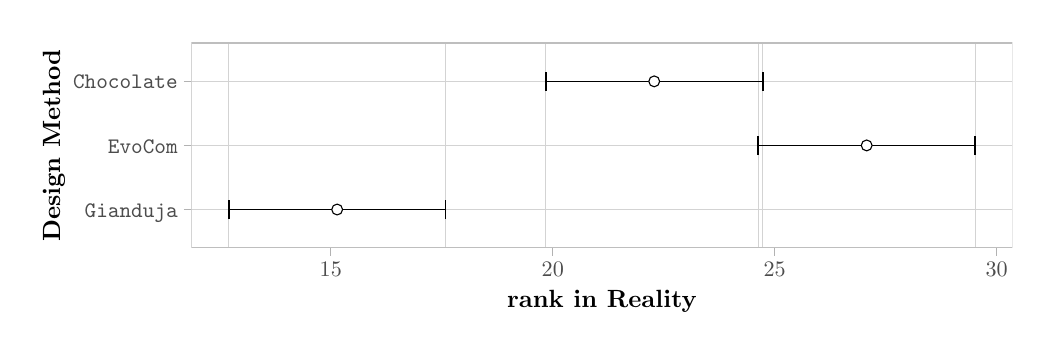
\begin{tikzpicture}[x=1pt,y=1pt]
\definecolor{fillColor}{RGB}{255,255,255}
\path[use as bounding box,fill=fillColor,fill opacity=0.00] (0,0) rectangle (361.35,108.41);
\begin{scope}
\path[clip] (  0.00,  0.00) rectangle (361.35,108.40);
\definecolor{drawColor}{RGB}{255,255,255}
\definecolor{fillColor}{RGB}{255,255,255}

\path[draw=drawColor,line width= 0.6pt,line join=round,line cap=round,fill=fillColor] (  0.00,  0.00) rectangle (361.35,108.40);
\end{scope}
\begin{scope}
\path[clip] ( 59.15, 28.81) rectangle (355.85,102.90);
\definecolor{fillColor}{RGB}{255,255,255}

\path[fill=fillColor] ( 59.15, 28.81) rectangle (355.85,102.90);
\definecolor{drawColor}{RGB}{211,211,211}

\path[draw=drawColor,line width= 0.3pt,line join=round] ( 59.15, 65.86) --
	(355.85, 65.86);

\path[draw=drawColor,line width= 0.3pt,line join=round] ( 59.15, 42.70) --
	(355.85, 42.70);

\path[draw=drawColor,line width= 0.3pt,line join=round] ( 59.15, 89.01) --
	(355.85, 89.01);

\path[draw=drawColor,line width= 0.2pt,line join=round] (265.60, 28.81) -- (265.60,102.90);

\path[draw=drawColor,line width= 0.2pt,line join=round] (342.36, 28.81) -- (342.36,102.90);

\path[draw=drawColor,line width= 0.2pt,line join=round] (151.02, 28.81) -- (151.02,102.90);

\path[draw=drawColor,line width= 0.2pt,line join=round] (187.21, 28.81) -- (187.21,102.90);

\path[draw=drawColor,line width= 0.2pt,line join=round] (263.97, 28.81) -- (263.97,102.90);

\path[draw=drawColor,line width= 0.2pt,line join=round] ( 72.63, 28.81) -- ( 72.63,102.90);
\definecolor{drawColor}{RGB}{0,0,0}

\path[draw=drawColor,line width= 0.6pt,line join=round] (265.60, 85.54) --
	(265.60, 92.49);

\path[draw=drawColor,line width= 0.6pt,line join=round] (265.60, 89.01) --
	(187.21, 89.01);

\path[draw=drawColor,line width= 0.6pt,line join=round] (187.21, 85.54) --
	(187.21, 92.49);

\path[draw=drawColor,line width= 0.6pt,line join=round] (342.36, 62.38) --
	(342.36, 69.33);

\path[draw=drawColor,line width= 0.6pt,line join=round] (342.36, 65.86) --
	(263.97, 65.86);

\path[draw=drawColor,line width= 0.6pt,line join=round] (263.97, 62.38) --
	(263.97, 69.33);

\path[draw=drawColor,line width= 0.6pt,line join=round] (151.02, 39.23) --
	(151.02, 46.17);

\path[draw=drawColor,line width= 0.6pt,line join=round] (151.02, 42.70) --
	( 72.63, 42.70);

\path[draw=drawColor,line width= 0.6pt,line join=round] ( 72.63, 39.23) --
	( 72.63, 46.17);

\path[draw=drawColor,line width= 0.4pt,line join=round,line cap=round,fill=fillColor] (226.40, 89.01) circle (  1.96);

\path[draw=drawColor,line width= 0.4pt,line join=round,line cap=round,fill=fillColor] (303.17, 65.86) circle (  1.96);

\path[draw=drawColor,line width= 0.4pt,line join=round,line cap=round,fill=fillColor] (111.83, 42.70) circle (  1.96);
\definecolor{drawColor}{RGB}{190,190,190}

\path[draw=drawColor,line width= 0.6pt,line join=round,line cap=round] ( 59.15, 28.81) rectangle (355.85,102.90);
\end{scope}
\begin{scope}
\path[clip] (  0.00,  0.00) rectangle (361.35,108.41);
\definecolor{drawColor}{gray}{0.30}

\node[text=drawColor,anchor=base east,inner sep=0pt, outer sep=0pt, scale=  0.80] at ( 54.20, 63.10) {\texttt{EvoCom}};

\node[text=drawColor,anchor=base east,inner sep=0pt, outer sep=0pt, scale=  0.80] at ( 54.20, 39.95) {\texttt{Gianduja}};

\node[text=drawColor,anchor=base east,inner sep=0pt, outer sep=0pt, scale=  0.80] at ( 54.20, 86.26) {\texttt{Chocolate}};
\end{scope}
\begin{scope}
\path[clip] (  0.00,  0.00) rectangle (361.35,108.41);
\definecolor{drawColor}{gray}{0.70}

\path[draw=drawColor,line width= 0.3pt,line join=round] ( 56.40, 65.86) --
	( 59.15, 65.86);

\path[draw=drawColor,line width= 0.3pt,line join=round] ( 56.40, 42.70) --
	( 59.15, 42.70);

\path[draw=drawColor,line width= 0.3pt,line join=round] ( 56.40, 89.01) --
	( 59.15, 89.01);
\end{scope}
\begin{scope}
\path[clip] (  0.00,  0.00) rectangle (361.35,108.41);
\definecolor{drawColor}{gray}{0.70}

\path[draw=drawColor,line width= 0.3pt,line join=round] (109.54, 26.06) --
	(109.54, 28.81);

\path[draw=drawColor,line width= 0.3pt,line join=round] (189.74, 26.06) --
	(189.74, 28.81);

\path[draw=drawColor,line width= 0.3pt,line join=round] (269.94, 26.06) --
	(269.94, 28.81);

\path[draw=drawColor,line width= 0.3pt,line join=round] (350.14, 26.06) --
	(350.14, 28.81);
\end{scope}
\begin{scope}
\path[clip] (  0.00,  0.00) rectangle (361.35,108.41);
\definecolor{drawColor}{gray}{0.30}

\node[text=drawColor,anchor=base,inner sep=0pt, outer sep=0pt, scale=  0.80] at (109.54, 18.35) {15};

\node[text=drawColor,anchor=base,inner sep=0pt, outer sep=0pt, scale=  0.80] at (189.74, 18.35) {20};

\node[text=drawColor,anchor=base,inner sep=0pt, outer sep=0pt, scale=  0.80] at (269.94, 18.35) {25};

\node[text=drawColor,anchor=base,inner sep=0pt, outer sep=0pt, scale=  0.80] at (350.14, 18.35) {30};
\end{scope}
\begin{scope}
\path[clip] (  0.00,  0.00) rectangle (361.35,108.41);
\definecolor{drawColor}{RGB}{0,0,0}

\node[text=drawColor,anchor=base,inner sep=0pt, outer sep=0pt, scale=  0.90] at (207.50,  7.44) {\bfseries rank in Reality};
\end{scope}
\begin{scope}
\path[clip] (  0.00,  0.00) rectangle (361.35,108.41);
\definecolor{drawColor}{RGB}{0,0,0}

\node[text=drawColor,rotate= 90.00,anchor=base,inner sep=0pt, outer sep=0pt, scale=  0.90] at ( 11.71, 65.86) {\bfseries Design Method};
\end{scope}
\end{tikzpicture}
